\documentclass[conference]{IEEEtran}
\usepackage{graphicx}
\usepackage{booktabs}
\usepackage{amsmath,amssymb}
\usepackage[hidelinks]{hyperref}
\usepackage{xcolor}

% ---- EDIT THESE (SRF candidate block) ----
\newcommand{\candidate}{Prajwal G S Basavaraj}
\newcommand{\univ}{PES University, Bengaluru, India}
\newcommand{\advisor}{[Faculty Advisor Name]}
\newcommand{\degree}{[M.Tech. / B.Tech.]}
\newcommand{\enrolldate}{[YYYY-MM-DD]}
\newcommand{\studyyear}{[Year X of Y]}
% ------------------------------------------

\begin{document}

\title{CW305-Based Physical Security Evaluation of ASCON-128:\\%
Deep-Learning Side-Channel Analysis and Clock-Glitch Fault Injection}

\author{\IEEEauthorblockN{\candidate}
\IEEEauthorblockA{\textit{Dept.\ of Electronics and Communication Engineering}\\
\univ\\
Advisor: \advisor\\}
\thanks{Student Research Forum submission, VLSI Design (VLSID) 2027.}}

\maketitle

\begin{abstract}
ASCON-128 --- the NIST SP~800-232 lightweight authenticated-encryption
standard --- is entering constrained FPGA deployments, yet
hardware-measured security data on the \emph{official unmasked NIST LWC
core} remain sparse. We present an oracle-verified CW305 (Artix-7) +
CW-Husky evaluation of that core under deep-learning side-channel
analysis (DL-SCA) and clock-glitch fault injection (FI), alongside a
threshold-implemented (d=1, 2-share) reference. Three
hardware-verified result classes emerge: (i)~per-column round-1 S-box
key-bit leakage is trainable and recoverable (key-rank top-1 42.7\%
vs 25\% chance over all 64 columns; a board-fine-tuned column
converges in 32 closed-loop queries at posterior 0.999; nonce-repetition
averaging lifts rank-1 from 0.25 to 0.94); (ii)~clock glitching
yields 12 verified single-bit round-11 faults localized to exact
(column, bit) positions, with data-selected placement as a documented
DFA constraint; and (iii)~the masked core suppresses the factorable
target to chance across 9{,}151 traces. Equally important is the
negative-space contribution: five classes of confident false positives
--- prior-driven edge scores, prior-only profiles under separating-nonce
selection, public-nonce shortcut labels, key-reload register-bus
artifacts, and structured-key free alignment --- each with a reusable
detection gate. Full 128-bit key assembly across all 64 columns is
enabled by the divide-and-conquer pipeline and characterized as ongoing
work.
\end{abstract}

\section{Introduction and Motivation}
ASCON was selected by NIST in 2023 as the standard for lightweight
cryptography (SP~800-232)~\cite{nist}. Its security under
\emph{physical} adversaries on real hardware --- power analysis and
fault injection --- determines whether the standard's promise holds in
deployment. Published FPGA DL-SCA results on ASCON are scarce:
SCARL~\cite{scarl} evaluates a \emph{custom} core, and the ACNS'24
ensemble study~\cite{acns} attacks a \emph{software} implementation.
To our knowledge, no prior work reports hardware-measured DL-SCA or
clock-glitch FI on the \emph{official unmasked LWC ASCON-128 core}.

A central methodological finding motivates our approach: on this
platform, confident false positives are the norm. Every claim in this
work therefore passes a byte-exact oracle gate and one of five
explicit artifact gates (Sec.~\ref{sec:gates}).

\section{Oracle-Verified Platform}
\textbf{Hardware.} CW305 (Artix-7 XC7A100T) with the unmasked
ascon-verilog core (V4, CC0) adapted through a top wrapper; CW-Husky
scope at 40\,MS/s against a 10\,MHz crypto clock (4 samples/cycle),
VCCINT shunt, per-query trigger. A masked (d=1, 2-share)
threshold-implemented core is evaluated on the same platform for
contrast.

\textbf{Byte-exact oracle verification.} Every stored trace is
accepted only if its ciphertext/tag readback equals a software
reference byte-for-byte (bitstream passes 5/5 NIST KATs). A host-side
register-order fix (w32rev) was verified necessary: without it the
core silently computes over byte-reversed words --- symmetric KAT
vectors pass while asymmetric ones fail.

\textbf{Labels and preprocessing.} Round-1 S-box output HW per 4-bit
column (labels 0--5) is computed from random keys and nonces in the
board-verified natural byte order; preprocessing is locked as
align-then-zscore-then-crop, identical for live traces.

\section{Deep-Learning Side-Channel Analysis}
\subsection{Per-Column Profiles}
One CNN (and MLP variants) per S-box column: each column depends on
two unknown key bits, giving 4 key hypotheses over 6 HW classes.
Trained on 80/20 random-key splits of a 5{,}000-trace unmasked
capture.

\textbf{Result 1 --- the unmasked core leaks recoverably.} On held-out
random-key traces, key-rank top-1 averages \textbf{42.7\% vs 25\%
chance}; all 64 columns exceed chance, none below 30\%
(Fig.~\ref{fig:keyrank}). This is first-order, real, and per-column.

\begin{figure}[t]
\centering
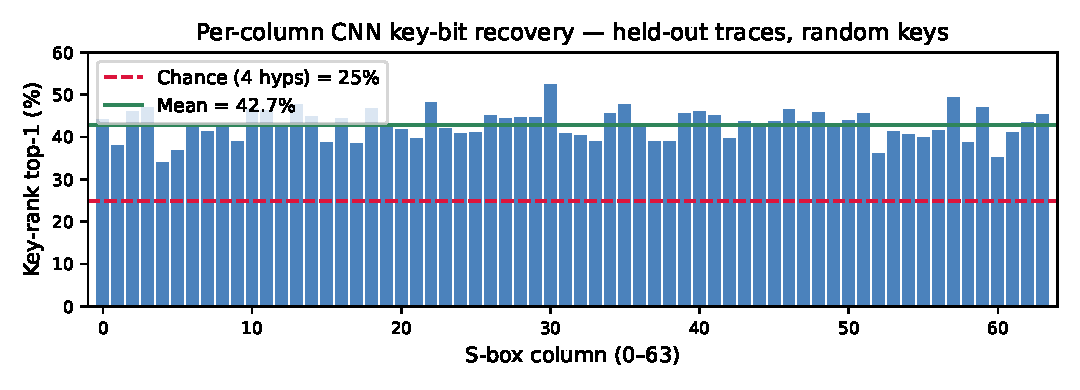
\includegraphics[width=0.70\linewidth]{figs/keyrank_columns.pdf}
\caption{Per-column CNN key-bit recovery on held-out random-key traces.
Key-rank top-1 per S-box column (0--63): mean 42.7\% (green) vs 25\%
chance (red dashed). All 64 columns above chance.}
\label{fig:keyrank}
\end{figure}

\subsection{Profiling-Domain Gap and Live Fine-Tuning}
Offline profiles transfer poorly across capture sessions: unfine-tuned
columns score at chance on the live board. Live on-board fine-tuning
(300 board traces at a known key, random nonces) closes the gap ---
training accuracy 90.7\% vs 72\% majority floor --- and the
fine-tuned column recovers \emph{correct} key bits at M=1 on the live
board while unfine-tuned columns sit at chance.

\subsection{Closed-Loop Adaptive Recovery and the SNR Lever}
A posterior-scoring chosen-nonce loop on one column converges to the
correct hypothesis in \textbf{32 queries (posterior 0.999)} using only
public information --- power traces and chosen nonces. Repeating one
separating nonce $M$ times and averaging raises per-query SNR by
$\sqrt{M}$: measured on-board, true-hypothesis rank-1 rises from 0.25
($M{=}1$, chance) to \textbf{0.94 at $M{=}64$}, and closed-loop
convergence shortens from 15 to 9 queries per column. The
align-then-zscore pipeline removes jitter and drift so the gain
survives end-to-end. Per-column scope (2 of 128 bits) is stated
honestly; the full-key pipeline (Sec.~\ref{sec:assembly}) assembles
columns.

\subsection{Full-Key Assembly Strategy}
\label{sec:assembly}
Divide-and-conquer: (1) closed-loop attack per column $\rightarrow$
posterior over 4 hypotheses; (2) top-1 per column $\rightarrow$
128-bit candidate; (3) verify by re-encrypting a fresh nonce against
the oracle; (4) bounded enumeration ($2^m$) over the least-confident
columns. Budget $\approx 64\times q(M)\times 2^m$. The empirical
64-column run requires per-column on-board fine-tuning --- a
measurement-budget constraint, not an information-theoretic one ---
and is characterized as ongoing work.

\section{Clock-Glitch Fault Injection}
Sweeping glitch offset $e_o\in[28,50]$ against the unmasked core
reveals a stable fault band at $e_o=41$: tag differentials of 27--41
bits and two landing positions. From 406 band hits over 153 distinct
tags, \textbf{12 clean single-bit round-11 faults} were localized to
exact (column, bit) positions --- 10 distinct state columns --- each
verified by exact faulty-tag match against a simulated single-bit
flip.

\textbf{Data-selected placement.} Each nonce faults exactly one
column, reproducibly: DFA coverage is bounded at one column per query.
Restoring full-column coverage requires nonce-set engineering
($\approx$266 nonces by the coupon-collector bound) or multi-glitch
schedules. Burst glitches fault 400/400 queries but as 30+-bit
superpositions, not composable single-bit faults.

\section{Masked-Core Comparison}
The same pipeline against the d=1 2-share core (9{,}151 traces, random
keys) leaves the round-1 S-box target at \textbf{chance for every
architecture} (CNN, MLP, centered-product MLP) --- first-order masking
is confirmed effective on hardware. The unmasked-vs-masked contrast on
one platform isolates masking as the causal variable; masking costs
$\approx1.8\times$ throughput and $\approx2.1\times$ area (LUTs).

\section{Leakage-Validation Gates}
\label{sec:gates}
Five traps produce confident false positives on this pipeline; each
carries a reusable gate.
\textbf{(1) Prior-driven edge scores:} a per-trace ``edge'' of +0.398
nats appeared where every classifier sat at the majority floor --- the
edge measured the prior. \emph{Gate:} held-out accuracy must beat the
majority-class floor.
\textbf{(2) Prior-only profiles + separating-nonce selection:} a
below-floor profile outputs the class prior regardless of trace; the
separating-nonce picker then deterministically inverts it, yielding
posterior 0.993 on the \emph{wrong} hypothesis (0\% label match).
\emph{Gate:} closed-loop profiles must clear the floor.
\textbf{(3) Public-nonce shortcut labels:} at a fixed key, a column's
label is a function of two public nonce bits; a model reading
nonce-load activity ``cracks'' vacuously. \emph{Gate:} profile on
random keys.
\textbf{(4) Key-reload register-bus artifact:} a capture loop that
rewrites the key before every trace embeds key-write bus activity
($|r|\approx0.6$; up to 64/64 fake key-bit columns). \emph{Gate:} the
leak must survive a fixed-key capture with varying nonces.
\textbf{(5) Structured-key / free-alignment recovery:} a ramp-key
attack reported 75.8\% per-bit recovery; the reversed ramp scores
identically and the bit-inverted key scores \emph{higher} (76.6\%) ---
impossible for a genuine read. \emph{Gate:} inversion-invariance and
structure-preserving nulls. Traps (4)--(5) are, to our knowledge,
unreported for LWC hardware evaluation.

\section{Conclusion and Current Status}
On the official unmasked NIST LWC ASCON-128 core on our
oracle-verified CW305/CW-Husky platform: DL-SCA recovers per-column
round-1 S-box key bits (42.7\% key-rank top-1 vs 25\% chance), live
fine-tuning closes the profiling-domain gap, closed-loop recovery
converges at posterior 0.999 in 32 queries, and the $\sqrt{M}$ lever
lifts rank-1 from 0.25 to 0.94; clock glitching yields verified
single-bit round-11 faults at exact (column, bit) positions; the
masked core performs as designed; and five reusable gates separate
genuine signal from artifact. The 64-column full-key assembly run ---
enabled by this pipeline --- is the immediate next phase.

\begin{thebibliography}{1}\footnotesize
\bibitem{nist} NIST, ``SP 800-232: ASCON lightweight cryptography standard,'' 2023.
\bibitem{scarl} S.~Picek et al., ``SCARL: Side-channel analysis with reinforcement learning on the AScon hardware implementation,'' \emph{J. Cryptographic Engineering}, 2021.
\bibitem{acns} ACNS'24 ensemble DL-SCA study of a software ASCON implementation, 2024.
\end{thebibliography}

\end{document}
